\documentclass{beamer}
\usetheme[numbering=none]{focus}

\usepackage{multicol}

\title{Dubbele bachelor Wiskunde Informatica}
\subtitle{Waarom zou een zinnig mens dat doen?}
\author{Jonas van der Schaaf}
\titlegraphic{
\includegraphics[scale=0.12]{assets/UvA_logo.png}}
\institute[UvA]{Universiteit van Amsterdam}
\date{\today}

\begin{document}
\begin{frame}
    \begin{center}
        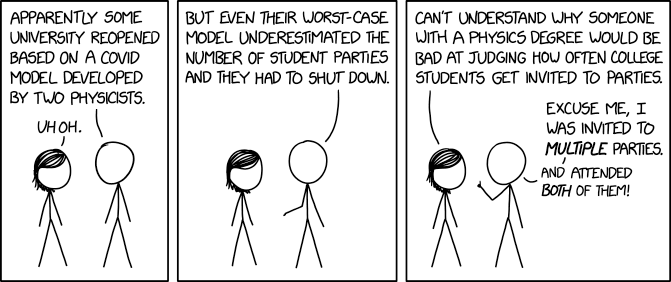
\includegraphics[scale=0.45]{assets/xkcd_parties.png}
    \end{center}
\end{frame}

\begin{frame}
    \maketitle
\end{frame}

\begin{frame}{Inhoud}
    \tableofcontents
\end{frame}

\section{Wie ben ik?}

\section{Wat is er zo leuk aan een dubbele bachelor?}

\section{Hoe ziet de dubbele bachelor Wiskunde Informatica er uit?}

\begin{frame}{Vakken}
    \begin{multicols}{2}
        Welke vakken doe je?
        \pause
        \begin{itemize}
            \item Grafentheorie
                  \pause
            \item Inleiding programmeren
                  \pause
            \item Datastructuren
                  \pause
            \item Calculus
                  \pause
            \item Lineaire algebra
                  \pause
            \item Analyse op de lijn
                  \pause
            \item Verzamelingen en getallen
                  \pause
            \item Programmeren en experimenteren
                  \pause
            \item Programmeertalen
                  \pause
            \item Numerieke Wiskunde
                  \pause
            \item Highlights Wiskunde
                  \pause
            \item Automaten en Formele Talen
                  \pause
            \item Logica en Onvolledigheid
                  \pause
            \item Kansrekening
                  \pause
            \item Differentiëren in meer dimensies
                  \pause
            \item Groepentheorie
                  \pause
            \item Multimedia
        \end{itemize}
        \pause
        Bijvakken?
        \pause
        \begin{itemize}
            \item Webtechnologie
                  \pause
            \item Itereren en visualiseren
        \end{itemize}
        \pause
        Honours?
        \begin{itemize}
            \pause
            \item Training BAPC
                  \pause
            \item Training IMC
                  \pause
            \item Differentiëren in meer dimensies, honours
                  \pause
            \item Groepentheorie, honours
        \end{itemize}
    \end{multicols}
\end{frame}
\end{document}